\section{Επισκόπηση Παραδειγμάτων Μαθημάτων}
\label{sec:example_courses_overview}

Η συλλογή \ENG{Golf Examples} χρησιμοποιείται ευρέως ως υλοποίηση αναφοράς για τη δοκιμή και την κατανόηση πακέτων \ENG{SCORM}, επειδή κάθε παράδειγμα απομονώνει ένα συγκεκριμένο τεχνικό χαρακτηριστικό του προτύπου~\cite{SCORMGolfExamples}. Για τους σκοπούς της παρούσας εργασίας επιλέγονται τέσσερα πακέτα: τα \ENG{\path{ContentPackagingSingleSCO_SCORM12.zip}} και \ENG{\path{RuntimeMinimumCalls_SCORM12.zip}} για το \ENG{SCORM} 1.2, καθώς και τα \ENG{\path{RuntimeMinimumCalls_SCORM20043rdEdition.zip}} και \ENG{\path{SequencingForcedSequential_SCORM20043rdEdition.zip}} για το \ENG{SCORM} 2004.

Η επιλογή αυτή δεν είναι τυχαία. Το πρώτο ζεύγος αντιστοιχεί άμεσα στις δύο βασικές διαστάσεις του \ENG{SCORM} 1.2 που αναλύθηκαν στις Ενότητες~\ref{subsec:scorm12_cam} και~\ref{subsec:scorm12_rte}, δηλαδή στο πακετάρισμα περιεχομένου και στην \ENG{run-time} επικοινωνία. Το δεύτερο ζεύγος επιτρέπει να φανεί πώς το \ENG{SCORM} 2004 διατηρεί τον ίδιο βασικό μηχανισμό εκκίνησης, αλλά τον επεκτείνει με πλουσιότερο μοντέλο δεδομένων και με τυπικό \ENG{sequencing}, όπως περιγράφηκε στις Ενότητες~\ref{subsec:scorm2004_rte} και~\ref{subsec:scorm2004_sn}.

Πέρα από την τεχνική τους αξία, τα παραδείγματα αυτά είναι χρήσιμα και επειδή το περιεχόμενό τους παραμένει οπτικά απλό. Οι σελίδες \ENG{HTML}, οι εικόνες και τα \ENG{JavaScript} αρχεία δεν κρύβουν την προδιαγραφή πίσω από βαρύ εκπαιδευτικό σχεδιασμό· αντίθετα, την καθιστούν ευανάγνωστη. Έτσι, ο αναγνώστης μπορεί να συνδέσει με σχετική ευκολία τις αφηρημένες έννοιες του Κεφαλαίου 3 με πραγματικά αρχεία, πραγματικά \ENG{identifiers} και πραγματικές κλήσεις μέσω \ENG{API}.

\subsection{Ενδεικτικό οπτικό υλικό από το περιεχόμενο}
\label{subsec:golf_example_visuals}

Το ίδιο το μαθησιακό περιεχόμενο των \ENG{Golf Examples} αποτελείται από απλές σελίδες \ENG{HTML} που συνοδεύονται από στατικές εικόνες και κοινά αρχεία μορφοποίησης. Τα αρχεία αυτά δηλώνονται ρητά στο \ENG{\texttt{imsmanifest.xml}} και φορτώνονται ως μέρος των αντίστοιχων \ENG{resources}. Το Σχήμα~\ref{fig:golf_example_content} παρουσιάζει τρεις χαρακτηριστικές εικόνες από το περιεχόμενο των ενοτήτων \ENG{Playing}, \ENG{Etiquette} και \ENG{Handicapping}, οι οποίες περιλαμβάνονται αυτούσιες στα πακέτα.

\begin{figure}[htbp]
\centering
\begin{subfigure}[t]{0.31\textwidth}
    \centering
    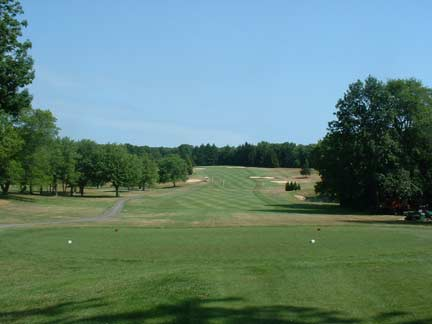
\includegraphics[width=\linewidth]{chapters/04_Example_Courses/figures/golf_playing.jpg}
    \caption{\ENG{Playing}}
\end{subfigure}
\hfill
\begin{subfigure}[t]{0.31\textwidth}
    \centering
    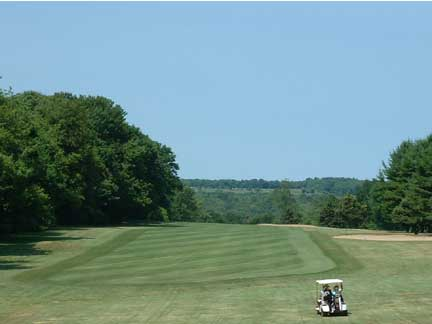
\includegraphics[width=\linewidth]{chapters/04_Example_Courses/figures/golf_course.jpg}
    \caption{\ENG{Etiquette}}
\end{subfigure}
\hfill
\begin{subfigure}[t]{0.31\textwidth}
    \centering
    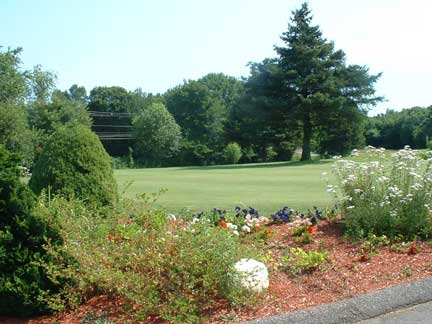
\includegraphics[width=\linewidth]{chapters/04_Example_Courses/figures/golf_handicapping.jpg}
    \caption{\ENG{Handicapping}}
\end{subfigure}
\caption{Ενδεικτικές εικόνες από το περιεχόμενο των \ENG{Golf Examples}}
\label{fig:golf_example_content}
\end{figure}

Η παρατήρηση αυτή έχει πρακτική σημασία. Οι εικόνες του Σχήματος~\ref{fig:golf_example_content} δεν αποτελούν εξωτερικό διακοσμητικό υλικό, αλλά τυπικούς πόρους περιεχομένου που δηλώνονται μέσα στο πακέτο, συνδέονται με συγκεκριμένα \ENG{HTML} αρχεία και συμμετέχουν στο ίδιο συμβόλαιο φορητότητας που αναλύθηκε στο Κεφάλαιο 3. Με άλλα λόγια, ακόμη και το απλό οπτικό υλικό υπάγεται στην ίδια λογική αυτοτέλειας του \ENG{PIF} και του \ENG{manifest}.
